\documentclass[border=4pt,12pt]{standalone}
% House style for redrawn exam diagrams (diagram-v4: 0.4pt lines, filled -latex arrows, fine dashes; stipple and hatching drawn as real dots/lines (no PDF/SVG patterns, so they render in every browser and at any scale); transparent background). Every figure \input's this.
\usepackage{amsmath,amssymb}
\usepackage{txfonts}
\usepackage{pdfrender,xcolor}
% \halo{text}: label on shading. The shading stops just around each letter's outline (a thin knock-out that follows the
% glyphs, like the papers' typesetting), never a box. Owner: "I don't want a box around the text".
\newcommand{\halo}[1]{\leavevmode\rlap{\pdfrender{TextRenderingMode=2,LineWidth=2.2pt,LineJoinStyle=1,StrokeColor=white,FillColor=white}#1}#1}
\usepackage{tikz,pgfplots}
\pgfplotsset{compat=1.18}
\usetikzlibrary{arrows.meta,calc,angles,quotes,patterns,patterns.meta,intersections,positioning,decorations.markings,shapes.geometric}
% Stipple and hatching are drawn as actual dots / lines clipped to the region (path picture), NOT as pattern fills:
% SVG <pattern> fills vanish or blur when browsers scale the image, so the owner could not see the shading.
% Each dot is a 0.72pt square (keeps SVGs small; reads as a dot at print size). Dots sit on one global staggered grid, so neighbouring regions line up.
\makeatletter
\newdimen\ex@x \newdimen\ex@y \newdimen\ex@xa \newdimen\ex@ya \newdimen\ex@xb \newdimen\ex@yb \newcount\ex@row
\def\exam@stipplecolor{black!75}\def\exam@dotr{0.42pt}\def\exam@dotgap{2.5}
\def\ex@rowdots{\ifdim\ex@x<\ex@xb \pgfpathrectangle{\pgfqpoint{\dimexpr\ex@x-0.36pt\relax}{\dimexpr\ex@y-0.36pt\relax}}{\pgfqpoint{0.72pt}{0.72pt}}\advance\ex@x by \exam@dotgap pt\relax\expandafter\ex@rowdots\fi}
\def\exam@stipple{%
  \pgftransformreset% dots are sized in real points even inside scaled pictures
  \pgfpointanchor{path picture bounding box}{south west}\ex@xa=\pgf@x \ex@ya=\pgf@y
  \pgfpointanchor{path picture bounding box}{north east}\ex@xb=\pgf@x \ex@yb=\pgf@y
  \pgfsetfillcolor{\exam@stipplecolor}\pgfmathsetmacro\ex@h{\exam@dotgap/2}%
  \pgfmathtruncatemacro\ex@r{floor(\ex@ya/\ex@h)-1}\ex@row=\ex@r\relax
  \ex@y=\ex@r\dimexpr\ex@h pt\relax
  \loop\ifdim\ex@y<\ex@yb
    \pgfmathtruncatemacro\ex@c{floor(\ex@xa/\exam@dotgap)-1}\ex@x=\ex@c\dimexpr\exam@dotgap pt\relax
    \ifodd\ex@row \advance\ex@x by \ex@h pt\fi
    \ex@rowdots
    \advance\ex@y by \ex@h pt \advance\ex@row by 1
    \ifnum\numexpr\ex@row-(\ex@row/4)*4\relax=0 \pgfusepath{fill}\fi% flush every 4 rows: bounded TeX memory, few clip copies in the SVG
  \repeat\pgfusepath{fill}}
\newdimen\ex@d
\def\exam@hatch#1{% #1 = 1 for /, -1 for \ ; lines 45 degrees, 3pt apart
  \pgftransformreset
  \pgfpointanchor{path picture bounding box}{south west}\ex@xa=\pgf@x \ex@ya=\pgf@y
  \pgfpointanchor{path picture bounding box}{north east}\ex@xb=\pgf@x \ex@yb=\pgf@y
  \ex@d=\dimexpr\ex@yb-\ex@ya\relax \ex@x=\dimexpr\ex@xa-\ex@d\relax
  \loop\ifdim\ex@x<\ex@xb
    \ifnum#1>0 \pgfpathmoveto{\pgfqpoint{\ex@x}{\ex@ya}}\pgfpathlineto{\pgfqpoint{\dimexpr\ex@x+\ex@d\relax}{\ex@yb}}%
    \else \pgfpathmoveto{\pgfqpoint{\ex@x}{\ex@yb}}\pgfpathlineto{\pgfqpoint{\dimexpr\ex@x+\ex@d\relax}{\ex@ya}}\fi
    \advance\ex@x by 4.24pt
  \repeat
  \pgfsetlinewidth{0.4pt}\pgfsetstrokecolor{black}\pgfusepath{stroke}}
\def\examstipple{\exam@stipple}\def\examhatch{\exam@hatch}\def\examsetstipplecolor#1{\def\exam@stipplecolor{#1}}\def\examsetdotgap#1{\def\exam@dotgap{#1}}
\makeatother
% (legacy pattern kept for old files)
% staggered stipple like the NESA papers' dotted shading
\pgfdeclarepatternformonly{exam stipple}{\pgfpointorigin}{\pgfqpoint{2.2pt}{2.2pt}}{\pgfqpoint{2.2pt}{2.2pt}}{%
  \pgfpathcircle{\pgfqpoint{0.55pt}{0.55pt}}{0.42pt}\pgfpathcircle{\pgfqpoint{1.65pt}{1.65pt}}{0.42pt}\pgfusepath{fill}}
\tikzset{
  every picture/.style={line width=0.6pt, >={Latex[length=2mm,width=1.3mm]}},
  curve/.style={line width=0.6pt},
  open arrow/.style={-{Latex[length=2mm,width=1.3mm]}},  % owner: filled -latex heads everywhere, no open chevrons
  aux/.style={dash pattern=on 2pt off 1.5pt, line width=0.6pt},
  shade/.code={\def\exA{#1}\def\exB{none}\ifx\exA\exB\else\pgfkeysalso{fill=black!18}\fi},
  shade/.default=on,
  shade dots/.style={fill=none, path picture={\examstipple}},
  stipple color/.code={\examsetstipplecolor{#1}},
  stipple gap/.code={\examsetdotgap{#1}},
  shade dense dots/.style={fill=none, stipple gap=1.6, path picture={\examstipple}},
  shade hatch/.style={fill=none, path picture={\examhatch{1}}},
  shade hatch reverse/.style={fill=none, path picture={\examhatch{-1}}},
  shade solid/.style={fill=black},
  pt/.style={circle, fill, inner sep=1.1pt},
  open pt/.style={circle, draw, fill=white, inner sep=1.1pt},
}
\pgfplotsset{
  exam axes/.style={axis lines=middle, axis line style={->}, xlabel={$x$}, ylabel={$y$},
    xlabel style={anchor=west}, ylabel style={anchor=south}, tick label style={font=\small},
    every axis plot/.append style={line width=0.6pt, black}, samples=200, clip=false,
    enlargelimits=false, axis on top},
}

\begin{document}
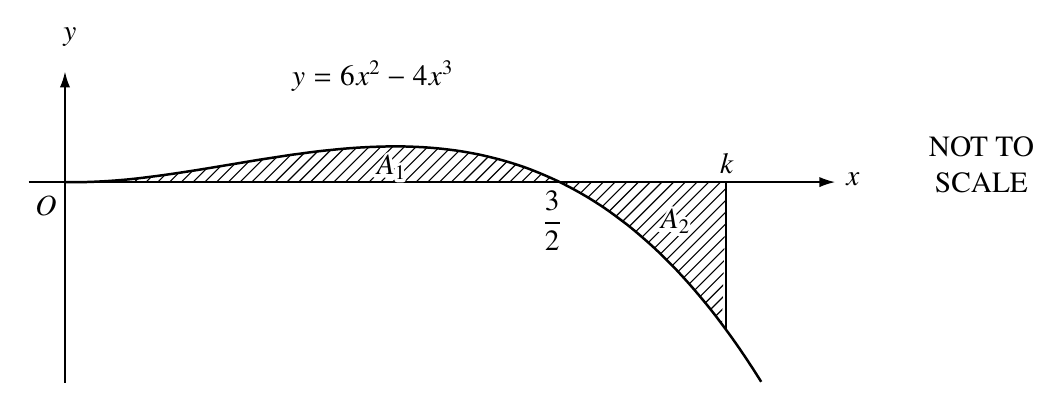
\begin{tikzpicture}[x=0.0127cm,y=-0.0127cm,font=\fontsize{10.6}{12.719999999999999}\selectfont]
\fill[shade hatch] plot[smooth] coordinates {(45.0,188.4) (52.8,188.6) (60.7,188.5) (68.5,188.4) (76.3,188.1) (84.2,187.7) (92.0,187.2) (99.8,186.6) (107.7,185.9) (115.5,185.1) (123.3,184.2) (131.1,183.2) (139.0,182.2) (146.8,181.1) (154.6,180.0) (162.5,178.8) (170.3,177.6) (178.1,176.4) (186.0,175.1) (193.8,173.8) (201.6,172.5) (209.5,171.2) (217.3,169.9) (225.1,168.6) (233.0,167.3) (240.8,166.0) (248.6,164.8) (256.4,163.6) (264.3,162.4) (272.1,161.2) (279.9,160.2) (287.8,159.1) (295.6,158.1) (303.4,157.2) (311.3,156.4) (319.1,155.6) (326.9,154.9) (334.8,154.3) (342.6,153.8) (350.4,153.4) (358.3,153.1) (366.1,152.9) (373.9,152.8) (381.8,152.8) (389.6,153.0) (397.4,153.3) (405.2,153.7) (413.1,154.3) (420.9,155.0) (428.7,155.9) (436.6,156.9) (444.4,158.1) (452.2,159.5) (460.1,161.0) (467.9,162.8) (475.7,164.7) (483.6,166.8) (491.4,169.1) (499.2,171.6) (507.1,174.3) (514.9,177.3) (522.7,180.5) (530.6,183.9) (538.0,188.5)}--cycle;
\fill[shade hatch] (538,188.5)--plot[smooth] coordinates {(538.4,187.5) (546.2,191.4) (554.0,195.5) (561.9,199.9) (569.7,204.5) (577.5,209.4) (585.4,214.6) (593.2,220.1) (601.0,225.9) (608.9,231.9) (616.7,238.3) (624.5,245.0) (632.4,252.0) (640.2,259.3) (648.0,267.0) (655.9,275.0) (663.7,283.4) (671.5,292.1) (679.3,301.2) (687.2,310.7) (695.0,320.5) (702.8,330.8)}--(707,188.5)--cycle;
\draw[line width=0.9pt] plot[smooth] coordinates {(45.0,188.4) (52.8,188.6) (60.7,188.5) (68.5,188.4) (76.3,188.1) (84.2,187.7) (92.0,187.2) (99.8,186.6) (107.7,185.9) (115.5,185.1) (123.3,184.2) (131.1,183.2) (139.0,182.2) (146.8,181.1) (154.6,180.0) (162.5,178.8) (170.3,177.6) (178.1,176.4) (186.0,175.1) (193.8,173.8) (201.6,172.5) (209.5,171.2) (217.3,169.9) (225.1,168.6) (233.0,167.3) (240.8,166.0) (248.6,164.8) (256.4,163.6) (264.3,162.4) (272.1,161.2) (279.9,160.2) (287.8,159.1) (295.6,158.1) (303.4,157.2) (311.3,156.4) (319.1,155.6) (326.9,154.9) (334.8,154.3) (342.6,153.8) (350.4,153.4) (358.3,153.1) (366.1,152.9) (373.9,152.8) (381.8,152.8) (389.6,153.0) (397.4,153.3) (405.2,153.7) (413.1,154.3) (420.9,155.0) (428.7,155.9) (436.6,156.9) (444.4,158.1) (452.2,159.5) (460.1,161.0) (467.9,162.8) (475.7,164.7) (483.6,166.8) (491.4,169.1) (499.2,171.6) (507.1,174.3) (514.9,177.3) (522.7,180.5) (530.6,183.9) (538.4,187.5) (546.2,191.4) (554.0,195.5) (561.9,199.9) (569.7,204.5) (577.5,209.4) (585.4,214.6) (593.2,220.1) (601.0,225.9) (608.9,231.9) (616.7,238.3) (624.5,245.0) (632.4,252.0) (640.2,259.3) (648.0,267.0) (655.9,275.0) (663.7,283.4) (671.5,292.1) (679.3,301.2) (687.2,310.7) (695.0,320.5) (702.8,330.8) (710.7,341.5) (718.5,352.5) (726.3,364.0) (734.2,376.0) (742.0,388.3)};
\draw[->] (9,188.5)--(816,188.5); \draw[->] (45.5,389)--(45.5,78);
\draw (707,188.5)--(707,336.5);
\node[anchor=base west,inner sep=0] at (43,47) {$y$};
\node[anchor=base west,inner sep=0] at (15,222) {$O$};
\node[anchor=base west,inner sep=0] at (825,192) {$x$};
\node[anchor=base west,inner sep=0] at (700,180) {$k$};
\node[anchor=base west,inner sep=0] at (272,92) {$y=6x^2-4x^3$};
\node[inner sep=0] at (533,227) {$\dfrac{3}{2}$};
\node[inner sep=0] at (372,174) {\halo{$A_1$}};
\node[inner sep=0] at (656,228) {\halo{$A_2$}};
\node[anchor=base west,inner sep=0] at (909,163) {NOT TO};
\node[anchor=base west,inner sep=0] at (915,199) {SCALE};\end{tikzpicture}
\end{document}
